% Chapter Template

\chapter{Implementation} % Main chapter title

\label{Chapter4} % Change X to a consecutive number; for referencing this chapter elsewhere, use \ref{ChapterX}

In this chapter, the overall structure of the project, how the files are arranged and the functionalities of each components, will be described in details.

%----------------------------------------------------------------------------------------
%	SECTION 
%----------------------------------------------------------------------------------------

\section{Files And Folders}

The folder names and file names are mostly self-explanatory or conventional in this project. They'll be described briefly in this section.

\begin{figure}[th]
\centering
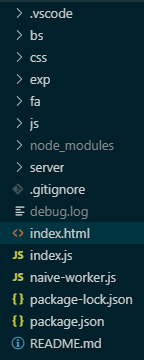
\includegraphics{Figures/Chapter4/filestructure.png}
\decoRule
\caption[File Structure]{A glimpse of files and folders.}
\label{fig:filestructure}
\end{figure}

\subsection{Folders}

\paragraph{Folder \texttt{./.vscode}}

The configured Visual Studio Code workspace settings file. This file is included and stored inside the workspace and only apply when the workspace is opened which overrides Visual Studio Code's default user settings. The author tweaked this file to make some parts of VS Code's editor, user interface, and functional behavior more fitting to review or to base future work upon this project\footnote{ To learn more about this file, see \url{https://code.visualstudio.com/docs/getstarted/settings}.}. 

VS Code provides two different scopes for settings:

\begin{itemize}
  \item User Settings - Settings that apply globally to any instance of VS Code you open.
  \item Workspace Settings - Settings stored inside your workspace and only apply when the workspace is opened.
\end{itemize}

Workspace settings override user settings\cite{bib:ms:vscode}.

\paragraph{Folder \texttt{./js}}

All the third-party open source \gls{js} dependencies are stored in this folder. Sometimes third-party open source projects include a bundle of \acrfull{js} and \gls{css} files, here only the pure \gls{js} projects' files are included.

\paragraph{Folder \texttt{./css}}

The \gls{css} files of the projects are included. Firstly there is a \\\texttt{./css/common.css} file, which sets the overall styles of the project, basically whatever the users can see at the very first glance when they open this project. Then there are several other \gls{css} files, each sets a specific portion of the styles in this project. These files include:

\begin{itemize}
\item \gls{css} File \texttt{./css/dock.css} sets the iOS-Dock look-like styles, making the focused item larger with larger margins and adjacent items smaller and smaller margins with their corresponding nearby items.
\item \gls{css} File \texttt{./css/minibar.css} sets the customed scrollbar styles that's being added upon the default styles of the dependency \emph{MiniBar} which is used to create custom scrollbars.
\item \gls{css} File \texttt{./css/stacked.css} sets the styles of the stacked cards effect.
\item \gls{css} File \texttt{./css/tabs.css} sets the related styles of the tabs effect.
\end{itemize}

Note that most of the effects require not only the \gls{css} stylings but also \gls{js} actions in order to work.

\paragraph{Folder \texttt{./fa}}

Assets of the dependency \emph{Font Awesome}, including all resources of the open source part. This dependency is used for the fonts of the icons in this project.

\paragraph{Folder \texttt{./bs}}

Assets of the open source project \emph{Bootstrap} by \emph{Twitter}. This dependency is used for the stylings of the web elements inside the control panel, such as input boxes, dropdown menus and font styles in control panel. It also comes with some nice utilities for general web elements style setting.

\paragraph{Folder \texttt{./node\_modules}}

Packages pulled from the \gls{js} dependency management tool \emph{npm}\footnote{ Build amazing things --- Essential JavaScript development tools that help you go to market faster and build powerful applications using modern open source code\cite{bib:npm:npm}. Too know more about \emph{npm}, see \url{https://www.npmjs.com/}.} are stored in this folder. The required dependency here is the package \texttt{minibarjs} under this folder -- in folder \texttt{./node\_modules/minibarjs}. Conventionally this folder shouldn't be included or committed to the version control system\footnote{ This is actually also what this project is following. }, because all the packages info are recorded in the file \texttt{package.json} and \texttt{package-lock.json} and if any dependencies are missing, running the \emph{npm} command \texttt{npm install} should be able to pull all necessary dependencies into this folder, however, considering this project sometimes can be run in an environment without internet connection, this folder is included in the final static zipped package.

\paragraph{Folder \texttt{./exp}}

Some trivial \emph{Python}, \gls{js} and \gls{html} codes left from the prototypes of implementation at the beginning of this project. Some of them are using different algorithms and different scripts trying to achieve similar results to this project. They are not in use anymore and only kept for future references.

\subsection{Top Level Files}

\paragraph{File \texttt{index.html}}

This entry \gls{html} file of this project. When a server is being run on the local machine, this is the first file getting executed. When a different implementation of the back end using techniques other than a web worker, for example a \texttt{WebSocket}, is developed and being adapted to this project, double-clicking on this file should also start this project.

\paragraph{File \texttt{index.js}}

The main \gls{js} script file of the project. This file gets included at the very end of the \gls{html} file \texttt{index.html}.

\paragraph{File \texttt{naive-worker.js}}

The back end calculation \gls{js} script. The only job of this script is to receive information of the image the front end is asking for, and post the result message back to the front end. This piece of scripts not only post the complete results back, but also slices of results when the calculation takes longer than a certain amount of time and let the front end decide what to do with the partial results\footnote{ In this project, what the front end will do after receiving partial results is that it will still render the slices of images onto the canvas and high light the painted partial image with green borders. }.

\paragraph{File \texttt{package.json}}

A description file of the \gls{js} package management tool \emph{npm}. This file can have many descriptions about what \emph{npm} should do for this workspace\footnote{ For for detailed information, see \url{https://docs.npmjs.com/files/package.json}.} but here it most importantly specifies which packages to pull from the global repository, in the \gls{json} field \texttt{'dependencies'}. Dependencies are specified in a simple object that maps a package name to a version range. The version range is a string which has one or more space-separated descriptors. Dependencies can also be identified with a tarball or git URL\cite{bib:npm:packagejson}.

\paragraph{File \texttt{package-lock.json}}

A generated file from \emph{npm} package manager which locks the version of the dependencies of this specific workspace. Take the current project as an example, in file \texttt{package.json} there is this part in the \gls{json} body:

\begin{verbatim}
{
  ..
  "dependencies": {
    ..
    "minibarjs": "^0.4.0",
    ..
  },
  ..
}
\end{verbatim}

This piece of code only specified that the version of the package \texttt{minibarjs} that we require will match all \texttt{0.x.x} releases including \texttt{0.5.x}, but will hold off on \texttt{1.x.x}. This file \texttt{package-lock.json} will ``lock'' the version inside current workspace to a specific version with a hashed fingerprint of the files, in the current project with a version number of \texttt{0.4.0} and a hash fingerprint \path{sha512-iCUE/YVWn+0ht+NV2fLBS8bAVxED/9l6A5i1qJ20csCrc0tXHamgpWCo7uL+23HQ0UyFPvpw1izw2l3vzVKkXg==}.

\paragraph{File \texttt{README.md}}

A brief introduction file for the global version control system \emph{GitHub}. Trivial.

\paragraph{File \texttt{.gitignore}}

Version control settings file, telling which files should not be committed to \emph{Git} system. Not relavant to the project but the version control during the development phase of this project. Trivial.

%----------------------------------------------------------------------------------------
%	SECTION 
%----------------------------------------------------------------------------------------

\section{Start the Project}\label{chap4:starttheproject}

Although this project is a pure web project, it cannot be started by simply double-clicking on the entry file \texttt{index.html}, because modern browsers usually don't not allow local scripts to directly start \emph{Web Worker}s\footnote{ Web Workers are a simple means for web content to run scripts in background threads.\cite{bib:moz:webworker}} for security concerns. However, \emph{Web Worker} is being used in this project as simple means for doing heavy calculations in background threads without interfering with the \gls{ui}, therefore, in order to start the project, a simple \gls{http} server must be up and running on the local machine.

It is also worth mentioning that this project should be running with Google Chrome browser as it supports most of the advanced visual effects and modern web technology syntax, known as \emph{HTML5}\footnote{ See \url{https://developer.mozilla.org/en-US/docs/Web/Guide/HTML/HTML5} for more detailed information.}. The recommended version of Google Chrome is \path{76.0.x}.

To start and keep a \gls{http} server running, the simplest and recommended way would be to use \emph{Python}'s \texttt{http.server}. To do that\cite{bib:moz:simplehttp}:

\paragraph{Install Python} If you are using \emph{Linux} or \emph{macOS}, it should be available on the system already. If you are a \emph{Windows} user, \emph{Python} installer can be downloaded from the \emph{Python} homepage and the instructions can be followed to install it:

\begin{itemize}
  \item Go to \url{python.org}
  \item Under the \emph{Download} section, click the link for \texttt{Python 3.xxx}.
  \item At the bottom of the page, choose the \emph{Windows x86 executable installer} and download it.
  \item When it has downloaded, run it.
  \item On the first installer page, make sure you check the \emph{``Add Python 3.xxx to PATH''} checkbox.
  \item Click \emph{Install}, then click \emph{Close} when the installation has finished.
\end{itemize}

\paragraph{Verification}

Open a \emph{Command Prompt} (Windows) / \emph{Terminal} (macOS / Linux). To check \emph{Python} is installed, enter the following command:

\begin{verbatim}
  python -V
\end{verbatim}

\paragraph{Navigation}

The above command should return a version number. If this is OK, navigate to the directory that the files of this project is inside, using the \texttt{cd} command.

\begin{verbatim}
  # include the directory name to enter it, for example
  cd Desktop/fractals
\end{verbatim}

\paragraph{Start the Server}

Enter the command to start up the server in that directory:

\begin{verbatim}
  # If Python version returned above is 3.X:
  python -m http.server
  
  # Or simply:
  py -m http.server

  # If Python version returned above is 3.X
  # and on non-Windows machines:
  python3 -m http.server

  # If Python version returned above is 2.X,
  # or if on macOS using the default Python
  # installed:
  python -m SimpleHTTPServer
\end{verbatim}

By default, the above actions will run the contents of the directory where the files of this project are located on a local web server, on port $8000$. In order to view this project now, simply go to this server by going to the \gls{url} \texttt{localhost:8000} in your web browser, to be specific and recommended in Google Chrome. Here the project entry \texttt{index.html} will be run by default and users can see directly the result.

%----------------------------------------------------------------------------------------
%	SECTION 
%----------------------------------------------------------------------------------------

\section{Front End}

Since this project is a pure web project, the front end occupies a large portion of the codes.

\subsection{HTML Entry \texttt{index.html}}

The entry of the project is where this program gets started, in similar concept of the \texttt{main()} function in \texttt{C} or the \texttt{public static void main(String[] args)} function in \texttt{Java}. The entry point is a \gls{html} file and as expected named \texttt{index.html}. It introduces the front end structure of the project in raw.

First part of the \gls{html} file is the \texttt{<head>} part. In this part, the character set of this web page is defined as \emph{UTF-8}, the size of the entire \gls{html} document as fullscreen size, scaling not allowed and not shrinking to display its content.

\begin{verbatim}
<meta charset="utf-8">
<meta name="viewport" content="width=device-width,
    initial-scale=1, shrink-to-fit=no">
\end{verbatim}

And then all the needed \gls{css} files are included to end the \texttt{<head>} part. Besides the \gls{css} files which will be described in \gmref{chap4:frontend-css}, the necessary \gls{css} files from third-party open source vendors are also included, including \emph{Bootstrap}'s \gls{css} part, \emph{FontAwesome} and \emph{MiniBar} \gls{css} assets.

The \texttt{<body>} part is the essential part of the \gls{html} entry, which describes the structure of what users can ``actually see''. It begins first with three \texttt{<div>} tags for the most important three parts of this project, the container for main background canvases, the container for mini-maps, and the container for the control panel floating on the top right corner of the \gls{ui} screen. The positioning, sizes and container behaviours of these \texttt{<div>}s are defined in the \gls{css} files which are already included. Before users set any effects up, these properties mostly come from the file \texttt{./css/common.css}.

\begin{figure}[th]
\centering
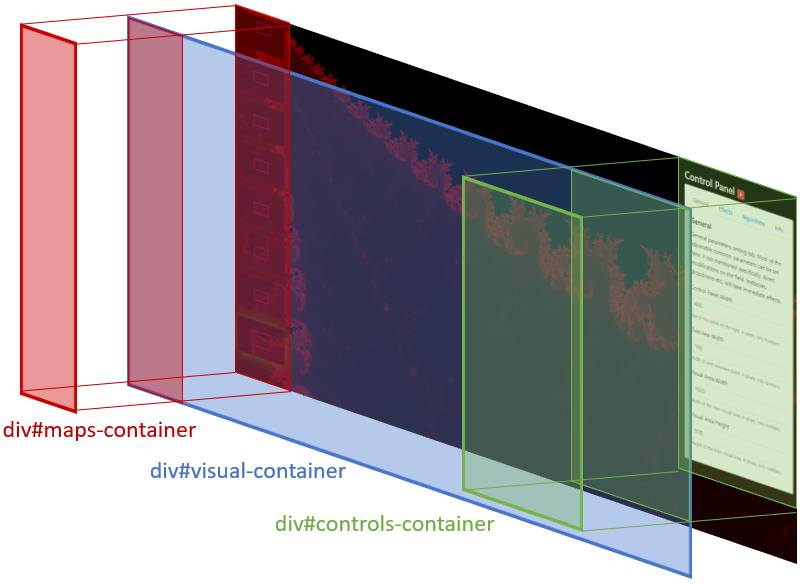
\includegraphics[width=\textwidth,keepaspectratio]{Figures/Chapter4/rootdom.png}
\decoRule
\caption[DOM Body Structure]{\gls{dom} structure in \texttt{<body>} tag.}
\label{fig:rootdom}
\end{figure}

After the visual \texttt{<div>} part, several \texttt{<script>} tags come after it to include what's necessary for the essential coding part. Here firstly are the dependencies of the project, including \emph{jQuery}, \emph{Bootstrap}'s \gls{js} part, and \emph{MiniBar}'s \gls{js} part. And then at the very end the main \gls{js} file \texttt{index.js} is included and all the core programs of this project goes in there.

Worth noting that conventionally all \gls{js} files should be included at the very end of the page as what we are doing now, unless the \gls{js} file is needed before the render phase of the web page. This way if the \gls{js} file is a little bit bigger than usual, the loading of the \gls{js} files won't affect the rendering process of the \gls{dom} documents.


\subsection{Main JavaScript \texttt{index.js}}

The main \gls{js} file \texttt{index.js} is where the core codes are. In this file there is firstly the definition of required classes from bottom level to the top, then the instantiation of them and putting the front end \gls{html} elements into action to display the overall results.

There in total four classes defined.

\subsubsection{Class \texttt{MandelWorker}}

The class \texttt{MandelWorker} is in charge of sending a message to the back end and when a result is sent back, handle it by executing a preset function(or say callback). This class is the red and green arrows shown in \gmref{fig:fpcpair}.

When instantiated, an instance of a native \emph{Web Worker} will also be created as a private property of this class. \texttt{MandelWorker} instantiates the \emph{Web Worker} by the script \texttt{naive\-worker.js}, which means that the script \texttt{naive\-worker.js} will be the core of the worker and this worker will be doing whatever in that script when it is asked to\footnote{ See \url{https://developer.mozilla.org/en-US/docs/Web/API/Web_Workers_API/Using_web_workers\#Spawning_a_dedicated_worker} for more detailed information of the process of instantiating a \emph{Web Worker}.}.

\textbf{Function \texttt{work(params...)}}

The function \texttt{work(params...)} is the interface between \texttt{MandelWorker} and the outside invoker. To get an image from the source, one must invoke this function with the needed parameters as follows:

\begin{itemize}
  \item \texttt{magnif} The magnification level of the result image to be expected from the \emph{Web Worker}.
  \item \texttt{centerX} The \texttt{x} component of the center coordinates on the mathmatical plane of the result image to be expected from the worker.
  \item \texttt{centerY} The \texttt{y} component of this coordinates.
  \item \texttt{width} The width in pixels of the result image.
  \item \texttt{height} The height in pixels of the result image.
  \item \texttt{callback} The function to execute when a result message is received.
  \item \texttt{callbackThis} The ``this'' context where the \texttt{callback} function should be executed under.
\end{itemize}

Here what's worth mentioning is the parameter \texttt{magnif}. The magnification level is a number representing the number of pixels that together has a length of $1$ on the mathmatical axis. As shown in \gmref{fig:magnif} is an image with the magnification level of $2$, since $2$ pixels have the length of $1$ on the mathmatical axis.

\begin{figure}[th]
\centering
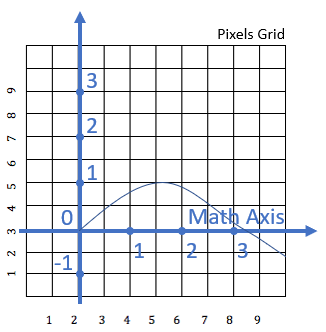
\includegraphics[keepaspectratio]{Figures/Chapter4/magnif.png}
\decoRule
\caption[Magnification Level]{Magnification level in aspect of mathmatical axis.}
\label{fig:magnif}
\end{figure}

Once this function is invoked, \texttt{MandelWorker} will tell its own \emph{Web Worker} to start working on datasets fetching\footnote{ In the context of the current project, is actually image generation. }, and if any sorts of results come through that worker, hit the \texttt{workerResponse(e)} function of the current \texttt{MandelWorker}.

\textbf{Function \texttt{workerResponse(e)}}

The function \texttt{workerResponse(e)} will be called when a response from the \emph{Web Worker} is sent back. It basically does one thing: checking if the parameters of \texttt{callback} and \texttt{callbackThis} were set when function \texttt{work(params...)} got invoked in the first place. If they were set to any function, call it under the conext of the parameter \texttt{callbackThis}.

\textbf{Function \texttt{destroy()}}

The function \texttt{destroy()} as the name implies is the method to destroy and release the resources for current \texttt{MandelWorker}. It terminates the \emph{Web Worker}, sets the response method to \texttt{null} so no responses will be dealt furthermore and sets all other references to \texttt{null} as well so the internal \gls{js} engine can garbage collect\footnote{ In computer science, garbage collection (GC) is a form of automatic memory management. The garbage collector, or just collector, attempts to reclaim garbage, or memory occupied by objects that are no longer in use by the program\cite{wiki:gc}.} all these instance to avoid memory leakage when the calculation gets heavy.

\subsubsection{Class \texttt{MapVisualPair}}

An abstract concept of pairing a minimap\footnote{ Same concept in current project as an \emph{overview}. } with an active focus region with higher resolution, as \gmref{fig:mapvisualpair} is an example of what they actually are respectively. This class is realizing the model of a pair of \gls{fpc} shown in \gmref{fig:fpcpair}.

\begin{figure}[th]
\centering
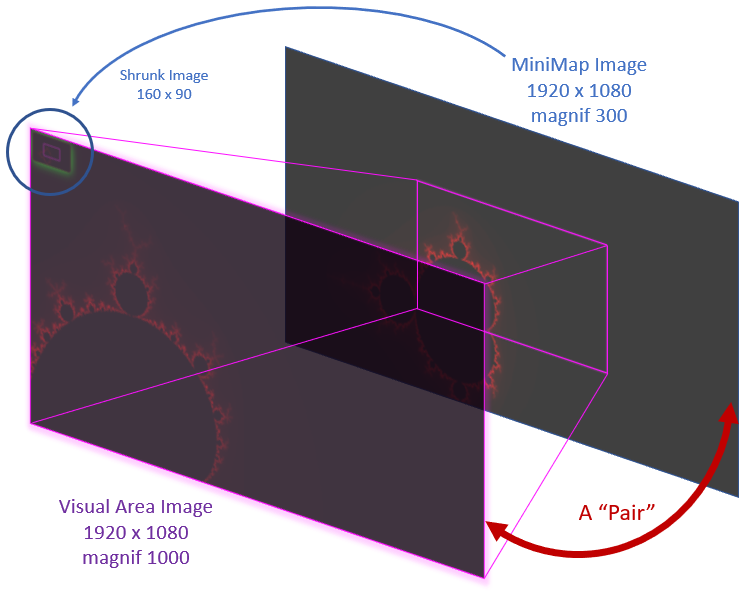
\includegraphics[width=\textwidth,keepaspectratio]{Figures/Chapter4/mapvisualpair.png}
\decoRule
\caption[Map Visual Pair]{Map area image and visual area(current focus region) image.}
\label{fig:mapvisualpair}
\end{figure}

The minimap representing a relatively ``larger'' area in the dataset and the visual area, which represents the active observing region, actually have both same resolution so they can both be displayed on a \gls{fhd} screen. Although the visual area seems ``smaller'' in comparison with the \gls{map} area, since it's an active region that is being observed by the user, the size of this visual area only represents its dimensions on the mathmatical plane and not smaller pixels-wise.

The \gls{map} image, however, will normally be shrunk and put on the left side of the screen, till the user hovers over a specific \gls{map} that will trigger the preview process of this program so he can have a glance of this image in a \gls{fhd} way.

The reason to pair up a visual area with a \gls{map} area is that whenever the user wants to browse around the dataset, the focusing coordinates on the visual area should also reflect back to the \gls{map} area, and the rectangle representing the current observing area should also get updated automatically. When there are more hierarchies of \glspl{map} present, this pairing mechanism becomes extremely helpful because the changes on the active region will flow all the way up to all levels of \glspl{map} necessary. Here \gmref{fig:mvp-pairflow} is a simple illustration of it.

\begin{figure}[th]
\centering
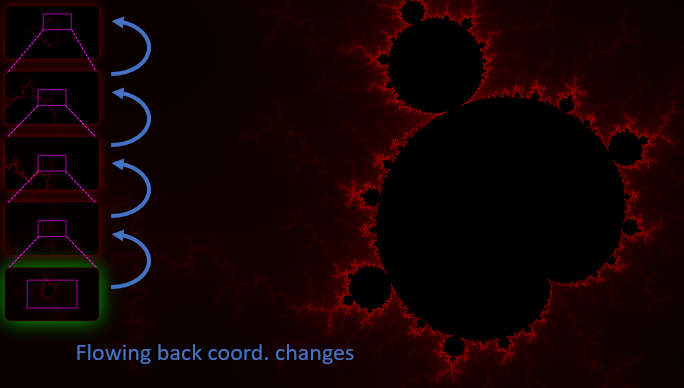
\includegraphics[width=\textwidth,keepaspectratio]{Figures/Chapter4/mvp-pairflow.png}
% 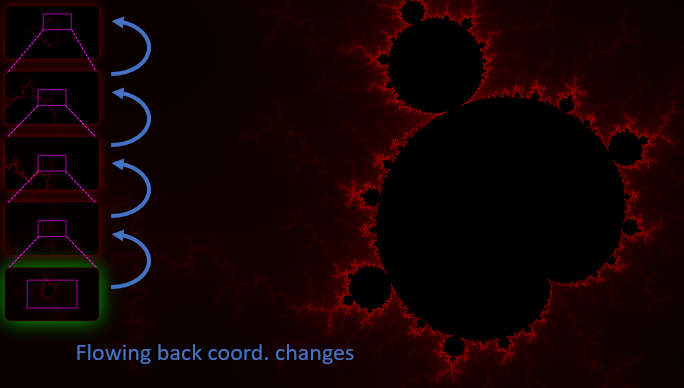
\includegraphics{Figures/Chapter4/mvp-pairflow.png}
\decoRule
\caption[Pairing Multiple Levels of \glspl{map}]{When multiple hierarchies of \glspl{map} present, visual area changes, all \glspl{map} changes.}
\label{fig:mvp-pairflow}
\end{figure}

\textbf{Function} \verb|init(mapCanvas, previewCanvas, visCanvas = null)|

This function will initialize the current \texttt{MapVisualPair}, bounding a \texttt{mapCanvas}, a \texttt{previewCanvas} and a \texttt{visCanvas} all of type \texttt{<canvas>} element to this class. When internally a drawing action should be performed, related images will be drawn on corresponding canvas.

The canvas \texttt{mapCanvas} will be used to draw the shrunk version of the \gls{map} image. \texttt{previewCanvas} will be used to draw the normal(\gls{fhd}) version of the \gls{map} image. And \texttt{visCanvas} will be used to draw the visual area image in \gls{fhd} if set.

After bounding the canvases, this function will also check if any event handlers are bound to the events \texttt{mouseover} and \texttt{mouseout} to the \texttt{mapCanvas} element, and record corresponding info to the element to avoid attemps to rebound event handlers to the same \texttt{<canvas>} element. In this way, only one event handler for \texttt{mouseover} and \texttt{mouseout} will be triggered when the user hovers their mouse on the \texttt{<canvas>} and when the user put their cursor out of the element.

The handlers this function is going to bound to the \texttt{mapCanvas} element are going to first add \gls{css} class \texttt{.nearby} to adjacent siblings of this canvas, and check if any additional callbacks this class should call. The callbacks, if any, which are set in the private properties \texttt{mouseOverCallback} and \texttt{mouseOutCallback}, will be called under set context \texttt{mouseOverCallbackThis} and \texttt{mouseOutCallbackThis} when user performs corresponding actions. As mentioned before, they will also be called only once because the bounding information is recorded. In the project, these callbacks and the contexts of them are set by a manager class \gmref{chap4:effectmanager}.

\textbf{Function} \verb|destroy()|

This function as the name implies releases all in-use resources, including \texttt{Worker}s, unbinding bound event handlers, clearing references to the canvases and their 2d contexts.

\textbf{Function} \verb|drawMapHoverArea(offsetRealX = 0, offsetRealY = 0)|

When the class is told to draw images on corresponding canvas elements, it will not automatically draw the purple rectangle indicating the current observing visual area, since the cached image data does not include this rectangle --- it doesn't belong to the extreme resolution dataset itself, therefore, this function exists to draw this current focus area using a purple rectangle to indicate it, drawing this rectangle on the \texttt{mapCanvas} whenever invoked. Note that whenever the image from the calculation side is fetched, without invoking this function, no current obeserving area rectangle will be shown, since the newly fetched image data will cover the old one also the old drawn rectangle.

The parameters \texttt{offsetRealX} and \texttt{offsetRealY} can also be set, as the purple rectangle to be drawn will then have an offset of (\texttt{offsetRealX}, \texttt{offsetRealY}) with respect to the center of the current observing area on the mathmatical complex plane.

\textbf{Function} \verb|drawPreviewHoverArea(offsetRealX = 0, offsetRealY = 0)|

Like the function \texttt{drawMapHoverArea}, this function will also draw a rectangle representing the current observing visual area, but on another canvas \texttt{previewCanvas}. The reason to separate these two functions is that the canvas \texttt{previewCanvas} isn't always visible and if these two functions are combined, it'll draw unintended purple rectangles on wrong canvases.

\textbf{Function} \verb|moveTo(x = null, y = null)|

This function is used to move the current \texttt{MapVisualPair} around. The parameters of coordinates are on the mathmatical complex plane, i.e. with respect to the entire datasets.

Note that these two parameters can be omitted and when omitted, the current \texttt{MapVisualPair} will simply send a ping to the calculation side and grab new image data for current observing coordinates, like a ``refresh'' action.

\textbf{Properties} \texttt{visMagnif} and \texttt{mapMagnif}

The magnification for the pair of these two canvases. See \gmref{fig:magnif} for the explanation of magnification level.

\textbf{Properties} \texttt{visCenterX} and \texttt{visCenterY}

The coordinates of the center point of the current observing visual area, with respect to the mathmatical complex plane.

\textbf{Properties} \texttt{visCanvasWidth} and \texttt{visCanvasHeight}

The width and height in \textbf{pixels} of the image data of the whole visual area. In \gmref{fig:mapvisualpair}, they're the dimensions of the whole visual area image. These properties have to exist because the dimensions of this area cannot always be fetched from the \texttt{visCanvas} property, as it is an optional parameter during the \texttt{init(params..)} phase and sometimes is absent.

\textbf{Properties} \texttt{visImgOffsetX} and \texttt{visImgOffsetY}

These two properties are set for the dragging actions that are realized in \gmref{chap4:minimapmanager}. They represents the current dragging offset with respect to the top left corner of the \texttt{visCanvas}. The reference point being top left corner not the center point is because in web canvas drawing system, the (0, 0) point is the top left corner, unlike in mathmatical complex plane it being the center.

\textbf{Properties} \texttt{mapCenterX} and \texttt{mapCenterY}

Like the properties \texttt{visCenterX} and \texttt{visCenterY}, these two properties represents the coordinates of the center point of the current \gls{map} area, with respect to the mathmatical complex plane. In \gmref{fig:mapvisualpair}, they're the center coordinates of the \gls{map} image.

\subsubsection{Class \texttt{MinimapManager}}\label{chap4:minimapmanager}

The manager class of all the minimaps, controlling all their behaviours on the top level. This class is described in \gmref{fig:fpcmanager}, the manager of all the \gls{fpc} models, plus a \gls{fhd} visual area.

\textbf{Inits}

\textbf{Function} \path{initMaps(visCanvas, previewCanvas, mapsContainer, visualContain er, hoverX = 0, hoverY = 0)}

This function initializes the states of all the \texttt{MapVisualPair}s that should be displayed, as well as initializing its own requird properties.

The properties \texttt{visCanvas} and \texttt{previewCanvas} are the canvases bound to this manager. \texttt{visCanvas} is the canvas for the main visual area and the details image is rendered on this canvas. \texttt{previewCanvas} is the canvas that's initially hidden, but will be shown when the \texttt{EffectManager} described in \gmref{chap4:effectmanager} instructs, designed for the presentation of the preview images. These two canvases have exactly the same dimensions, covering the entire \gls{ui} viewport, and on the most bottom layer of the page hence being laid over by the \glspl{map} and control panels. \texttt{previewCanvas} in turn lays over \texttt{visCanvas} since when a preview instruction is issued, it has to be displayed over the original visual area.

The property \texttt{mapsContainer} is the container holding all the canvases for the display of \glspl{map}. It's bound to this manager during this initialization phase. During this phase, step one, basic \gls{dom} structure of one \gls{map}, consisting of one \texttt{<cavans>} element and one \texttt{<span>} element for the purpose of showing the \texttt{magnif} number, will be created and appended to this container. The center coordinates of the \gls{map} will be from the parameters \texttt{hoverX} and \texttt{hoverY}, and \texttt{0} if not designated. The \texttt{magnif} level of the first \gls{map} comes from the variable \texttt{mapMagnif} in the global scope of \texttt{index.js}\footnote{ Technically not the global scope of entire \texttt{index.js} file per se, but the ``global scope'' of entire anonymous function that envelops all the codes.}. Based on the \texttt{magnif} of the first \gls{map} and the \texttt{visMagnif} variable defined in global scope, the initial dimensions of the focus area projected on the \gls{map} can be calculated.

With the dimensions of the first \gls{map}, this manager then decides whether additional \glspl{map} are required, based on the results of whether this projected area on \gls{map} is too small. If this area is too small, additional \gls{dom} structure consisting of one \texttt{<canvas>} and one \texttt{<span>} will be created and appended to the container. The criteria of whether this area is too small is defined by the private property \texttt{this.minStrokeW}\footnote{ In pixels.} of this manager. After the new \gls{dom} is created, we then will have two canvases. The first one will be the \gls{map} canvas and the one created after the calculation of the projection area will be the ``visual'' area. These two areas will then be paired up, forming an object of \texttt{MapVisualPair}. The \texttt{magnif} value of the visual area will be determined by the \texttt{magnif} value of the \gls{map} area, the minimal dimensions allowed for the projection area preset in \texttt{this.minStrokeW} and the dimensions of the dimensions of \texttt{previewCanvas}.

Since the model of \gls{fpc} are hierarchical, we can easily see that the new \texttt{magnif} value of the next \gls{map} area will be the value of the \texttt{magnif} value of the previous visual area. After the pairing of these two \glspl{map} and forming a first \texttt{MapVisualPair}, we can repeat this process described in above paragraph until the projection area on the current \gls{map} area is big enough then set in \texttt{this.minStrokeW}. When this happens, we bind the most recent \gls{map} canvas with the main visual area canvas and form the final \texttt{MapVisualPair}. This pair is named \texttt{this.pairMain} in this manager.

And the end of the initialization process, we put all these generated \texttt{MapVisualPair}s in an array called \texttt{this.pairs} and also bind \texttt{visualContainer} which holds \texttt{visCanvas} and \texttt{previewCanvas} with this manager. Later this container will be used for the events binding of \gls{ui} interactions.

\textbf{Function} \verb|initPairMainDrag()|

This function is called after the process in \texttt{initMaps(params..)} is complete. It registers necessary event handlers for mouse dragging related events that allows for browsing around the center of the focus view like Google Maps, including:

\begin{itemize}
  \item \path{pairMainMouseDown(e)} is bound with what was set in \texttt{visContainer} property, responding to single mouse pressing event without releasing the button.
  \item \path{pairMainMouseMove(e)} is bound with what was set in \texttt{visContainer} property, responding to single mouse moving event without releasing the button.
  \item \path{pairMainMouseUp(e)} is bound with what was set in properties \texttt{visContainer} \textbf{or} anywhere on the web page, responding to single mouse button releasing event.
\end{itemize}

All the handlers are bound under the context of the current class, a.k.a \texttt{this} or \texttt{MinimapManager}.

\textbf{Function} \verb|initPairMainWheel()|

This function can be called after the process in \texttt{initMaps(params..)} is complete. In the project it is called after \texttt{initPairMainDrag()}. It registers necessary event handlers for mouse wheeling related events that allows zooming into the dataset on the fly like Google Maps. It binds the event handler \texttt{pairMainWheel(e)} to the mouse wheel event with the root document of the web page, which means when user tries to scroll the middle button of thier mouse, this handler will be triggered.

This handler is also bound under the context of the current class, a.k.a \texttt{this} or \texttt{MinimapManager}.

\textbf{Handlers and Functions Related with Mouse Dragging}

\textbf{Function} \path{pairMainMouseDown(e)}

As mentioned before, this function handles the event when user presses the left mouse button before releasing it.

When this event happens on the target, we first records the current position of the user's cursor on the attributes \texttt{dragStartX}, \texttt{dragStartY}, \texttt{dragCurrentMouseX} and \texttt{dragCurrentMouseY}, and use \texttt{window.requestAnimationFrame(callback)} to activate an animation with max frame rates allowed. The \texttt{callback} parameter in \path{window.requestAnimationFrame(callback)} is the method \texttt{pairMainStepDrag(timestamp)} of this manager and will be called every time when a new frame should be rendered to the screen and we use this mechanism to repaint the dragged image of the current focus area in the correct place.

This function also sets a \texttt{dragGlobalID} property to the class to mark that this process has been marked started.

\textbf{Function} \path{pairMainMouseMove(e)}

This function handles the situation when the user, while not releasing the left mouse button, moves the mouse around.

This function does one simple thing: if the \texttt{dragGlobalID} attribute is set on the class meaning the process of mouse dragging being started, set the current postion of user's cursor to the attributes \texttt{dragCurrentMouseX} and \texttt{dragCurrentMouseY} to be used by \texttt{pairMainStepDrag(timestamp)}.

\textbf{Function} \path{pairMainStepDrag(timestamp)}

During the phase of dragging, since this function is triggered every time a new frame is needed to be rendered, we simply grab the values in \texttt{dragCurrentMouseX} and \texttt{dragCurrentMouseY}, and compare them with \texttt{dragStartX} and \texttt{dragStartY}, and see how much the user has moved their mouse since the last frame rendered.

We then paint the image based on the offsets we calculated from these two pairs of values on the correct position.

\textbf{Function} \path{pairMainMouseUp(e)}

When user releases the mouse button after the series of the previous events, this handler gets triggered.

We repaint the image of the focus area one last time on the correct place, and put this final offset on the properties \texttt{visImgOffsetX} and \texttt{visImgOffsetY} of \texttt{this.pairMain}, and stop the animation using \texttt{window.cancelAnimationFrame(this.dragGlobalID)} with the help of the recorded \texttt{dragGlobalID}.

At this point, new coordinates of the current center of visual view will be calculated and check how many of the \texttt{MapVisualPair}s need updates. All of those that need updates will be instructed to send requests to back end resolver and fetch new image data.

The properties \texttt{visImgOffsetX} and \texttt{visImgOffsetY} are set on \texttt{this.pairMain} so next time when user starts to drag the mouse, the image of the visual area will start from the current offset and not jump back to the initial offset of this drag which is \texttt{(0, 0)}, even if the calculation from the resolver hasn't completed yet. This mechanism can be compared with this situation of Google Maps: when user is looking at location $A$ and the loading is completed, and drags the map around and stops at another location $B$, the map will start to fetch the data around location $B$. However, if the user refuses to wait and starts to drag again to a new location $C$, the second drag starts from location $B$ and not location $A$.

\textbf{Handlers and Functions Related with Zooming In and Out}

\textbf{Function} \path{pairMainWheel(e)}

This function handles the event when user scrolls the middle button of their mouse.

In this handler, we first check if this process is already ongoing or not.

If this process hasn't been started yet, we set a property \texttt{wheelCurrentRatio} representing how much user has zoomed in to \texttt{1}, and records the current \texttt{magnif} value of the visual area, \texttt{visMagnif}. We then request a same rendering mechanism trigger by \texttt{window.requestAnimationFrame} and pass on the frame executor \path{pairMainStepWheel (timestamp)} to start an animation for zooming in. After that, while the zooming animation of the current visual area image is ongoing, we set a timer of $500$ milliseconds that detects if the scrolling on the mouse button is still happening. When the timer hits, meaning within $500$ milliseconds the user hasn't scrolled the mouse button, we should consider that user wants to stop the zooming at current depth.

If this process is started already, meaning this process is still ongoing, we only refresh the counter of the timer, and reset it back to $500$ milliseconds and let the \texttt{pairMainStepWheel(timestamp)} to keep working on each frames of the animation.

\textbf{Function} \path{pairMainStepWheel()}

During the phase of zooming in or out of the dataset, this function is triggered every time a new frame is needed to be rendered. We check if the zooming direction is in or out, then repaint the zoomed image and calculate the new \texttt{visMagnif}\footnote{ As mentioned before, the \texttt{magnif} value of the main visual area.}.

\textbf{Function} \path{pairMainTimeoutWheel()}

If this function gets triggered, it means the timer has timed out and user wants to stop at current depth. Since each frame we have the value of \texttt{visMagnif} calculated, we now have a new \texttt{magnif} value for the visual area in the system. 

To make the current system has the clear resolution again, two situation can happen: user has either zoomed deeper into the dataset, or has zoomed out shallower.

When the first situation is the case, we start from the most zoomed in \gls{map}, and check whether with its \texttt{magnif} value new \glspl{map} are needed. This process is the same as described in \texttt{initMaps(params...)} since we're here also initializing new \glspl{map}, adding more to the pile of \texttt{this.pairs}.

When the second situation is the case, we do the reverse way of the initializing process. If the current projection area is larger than the most zoomed in \gls{map} entirely, this \gls{map} is no longer needed and needs to be removed. We delete this \gls{map}, invoking all the \texttt{destroy()} methods on \texttt{MapVisualPair} and their \texttt{MandelWorker}s, and move one level upper. We stop at the level where the projection area is small enough within one \gls{map}, and reconnect the current most zoomed in map with the canvas of the main visual area.

After the increment or decrement of the \glspl{map}, \texttt{MapVisualPair} that needs to get updates will be instructed to send requests to resolvers.

\subsubsection{Class \texttt{EffectManager}}\label{chap4:effectmanager}

This class manages the behaviours, activation and deactivation of the overview effects and the preview effects of the overviews.

General functions: \texttt{init()}, \texttt{getInfo(el)}

Fade in / out related functions: \texttt{fadeMouseOver(e, currentPair)}, \texttt{fadeMouseOut(e, currentPair)}

Zoom in / out through related functions: \texttt{zoomMouseOver(e, currentPair)}, \texttt{zoomStep(timestamp)}, \texttt{zoomMouseOut(e, currentPair)}

General preview effects functions: \texttt{updatePreview()}, \texttt{updateFadePreview()}, \texttt{updateZoomPreview()}, \texttt{destroyPreview()}

General overview effects functions: \texttt{destroy()}, \texttt{update()}

Scrollbar + Dock effects specific functions: \texttt{initScrollbar()}, \texttt{destroyScrollbar()}, \texttt{updateScrollbar()}

Stacked Cards effects specific functions: \texttt{initStacked()}, \texttt{destroyStacked()}, \texttt{updateStacked()}

Tabs effects specific functions: \texttt{initTabs()}, \texttt{destroyTabs()}, \texttt{updateTabs()}

\subsubsection{Instantiation, Variables and the Rest}

\begin{itemize}
  \item \texttt{screenWidth}
  \item \texttt{screenHeight}
  \item \texttt{mapWidth}
  \item \texttt{mapHeight}
  \item \texttt{controlPanelWidth}
  \item \texttt{visMagnif}
  \item \texttt{mapMagnif}
  \item \texttt{hoverX}
  \item \texttt{hoverY}
  \item \texttt{mainCanvas}
  \item \texttt{previewCanvas}
  \item \texttt{\$(`\#visual-container')}
  \item \texttt{\$(`\#maps-container')}
\end{itemize}

\subsection{CSSs for Overview Effects}
\label{chap4:frontend-css}

Folder \texttt{./css} includes five \gls{css} files, each setting up some visual effects of the project.

File \texttt{./css/common.css} first sets up all general appearance of the elements on the web page when no parameters or effects are set. File \texttt{./css/dock.css} sets up the appearance when \emph{Scrollbar + Dock} is activated, only the iOS Dock part and file \\\texttt{./css/minibar.css} sets up the scroll bar part. File \texttt{./css/stacked.css} sets up the effects of stacked cards. File \texttt{./css/tabs.css} sets up the effects of the tab selection on the top.

\subsection{Scrollbar + Dock Effect}

\subsection{Stacked Cards Effect}

\subsection{Tabs Effect}

%----------------------------------------------------------------------------------------
%	SECTION 
%----------------------------------------------------------------------------------------

\section{Back End Calculation}

The back end calculation is done in the \gls{js} file \texttt{naive-worker.js}. This file is being used for initializing the \emph{WebWorker}s inside \texttt{index.js} dynamically. Whenever a calculation or extraction for a specific region of a dataset is needed, the main \gls{js} file \texttt{index.js} is going to send a message to \texttt{naive-worker.js} with desired parameters and this back end will respond with corresponding image data.

\begin{figure}[th]
\centering
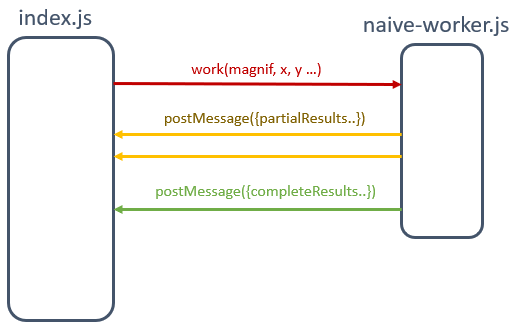
\includegraphics{Figures/Chapter4/messageexchange.png}
\decoRule
\caption[Message Exchange]{Message exchange between \texttt{index.js} and \texttt{naive-worker.js}.}
\label{fig:messageexchange}
\end{figure}

\subsection{Global Scope}

In the global scope of this file, the following things were done.

\paragraph{Includes} The \texttt{decimal.js} dependency is included for high-precision floating points calculation. Default parameters for the dependency is set.

\paragraph{Constants} Constants of default screen width and default screen height are defined in case the front end doesn't give these parameters.

\paragraph{Canvas} An \texttt{OffscreenCanvas} instance is created and instantiated with the dimensions of by default the values of the defined constants. The \texttt{OffscreenCanvas} will be used as the canvas to generate the desired image on, and since it's not being shown on the screen, will occupy less system resources and boost the calculation speed. Corresponding variables is declared after the instantiation, respectively \texttt{canvas} for the \texttt{OffscreenCanvas} itself and \texttt{ctx} as the 2d context of the canvas.

\subsection{Message Reception}

See \gmref{fig:messageexchange}.

\subsection{Iteration Limit}

\subsection{Iteration Count for One Point}

\subsection{Image Generation}

\subsection{High Precision Version}

%----------------------------------------------------------------------------------------
%	SECTION 
%----------------------------------------------------------------------------------------

\section{Utility Assets}

Other open source third-party utilities lie in different folders with corresponding names.

\subsection{Folder \texttt{./js}}

In \texttt{./js} folder, all \gls{js} third-party files are here, including:

\begin{itemize}
    \item File \texttt{decimal.min.js} is for high-precision floating points calculation for \acrfull{js}.
    \item File \texttt{jquery-3.4.1.min.js} is for \gls{dom} traversal and manipulation, event handling and animation.
    \item File \texttt{bootstrap.bundle.min.js} is for some basic styling of the control panel sitting on top right corner of the screen.
\end{itemize}

\subsection{Folder \texttt{./fa}}

\subsection{Folder \texttt{./bs}}

\subsection{Folder \texttt{./css}}